\subsection{Aplicaci�n}
\begin{frame}
\frametitle{}

\begin{figure}
\begin{tikzpicture}[node distance=0.5cm, auto,>=latex', thick]
\scriptsize
    % We need to set at bounding box first. Otherwise the diagram
    % will change position for each frame.
    \path[use as bounding box] (-1.5,0) rectangle (12,-2);

    % TT methodology     
    \node [phase]                        (monitoreo)     {Vigilancia};
    \node [phase, below of=monitoreo]    (choice)        {Elecci�n};
    \node [phase, below of=choice]       (acquisition)   {Adquisici�n};
    \node [phase, below of=acquisition]  (adaptation)    {Adaptaci�n};
    \node [phase, below of=adaptation]   (absortion)     {Absorci�n};
    \node [phase2,below of=absortion]    (aplication)    {Aplicaci�n};
    \node [phase, below of=aplication]   (difusion)      {Difusi�n};

    %%%%%%%%%%%%%%%%%%%%%%%%%%%%%%%%%%%%%%%%%%%%&
    %            Aplicaci�n
    %%%%%%%%%%%%%%%%%%%%%%%%%%%%%%%%%%%%%%%%%%%%&
    \node [ph_explain2, right=0.5cm of adaptation.east] (exp_aplication)    
    {
      \begin{center} \textbf{Proyecto Davinci} \end{center}
 
      \begin{itemize}
        \footnotesize
        \item Programa de la secretar�a de desarrollo econ�mico
         \begin{itemize}
          \footnotesize
          \item Transferencia de conocimiento en evaluaci�n tecnol�gica.
          \item Transformaci�n de resultados de la investigaci�n en innnovaciones del mercado.
          \item Se presentaron 85 investigaciones.
            \begin{itemize}
             \footnotesize
             \item Se generaron descriptivos tecnol�gicos 
             \item Se gener� el mapa de tecnolog�a para la siguiente etapa con 25 tecnolog�as.
            \end{itemize}
          \item Capacitaci�n en el seminario comportamental Embate (Emprendimiento de base tecnol�gica) \copyright.
            \begin{itemize}
             \footnotesize
             \item Selecci�n de los 10 mejores proyectos.
            \end{itemize}
         \end{itemize}
       \item Validaci�n empresarial de cara al mercado. Para revisar la pertinencia y aplicabilidad de los modelos de negocio construidos en la fase Diligencia de la Innovaci�n.
      \end{itemize}
    };

\end{tikzpicture}
\end{figure}
\end{frame}

\begin{frame}
 \begin{center} \textbf{Proyecto Smart Grids} \end{center}
     \only<1>{
       \begin{center} 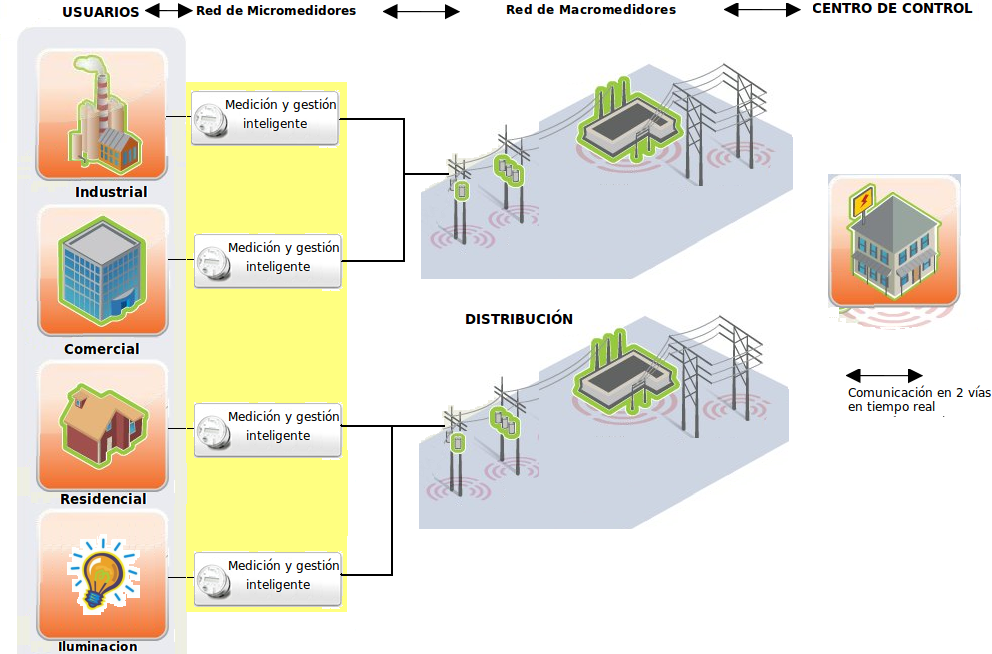
\includegraphics[scale=.45]{../images/smart_grid_propuesta.png} \end{center}
     }


\end{frame}
 

\begin{frame}

   \begin{center} \textbf{Proyecto SIEBOT} \end{center}
   \begin{center} 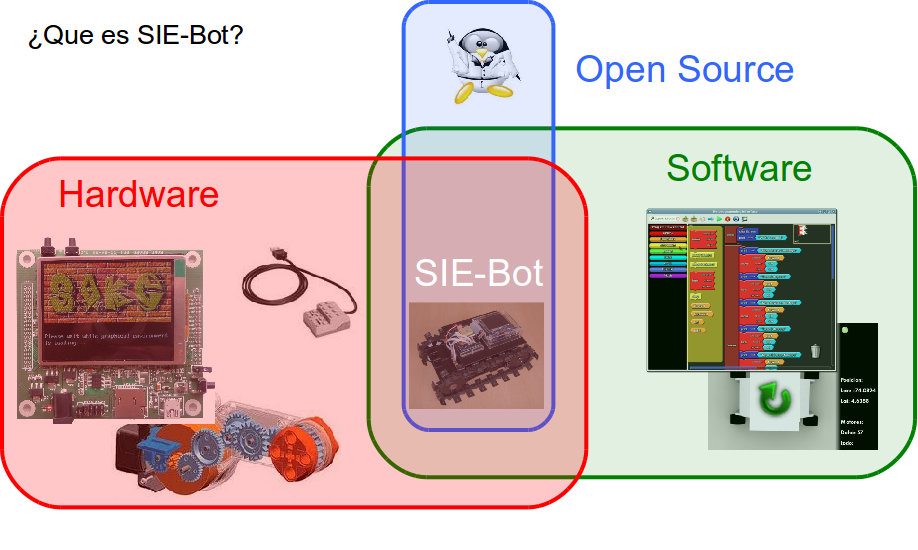
\includegraphics[scale=.3]{../images/siebot1} \end{center} 
   \begin{center} 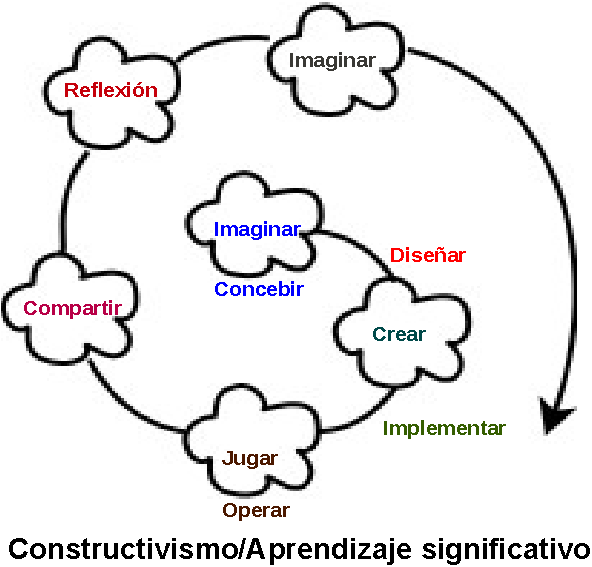
\includegraphics[scale=.45]{../images/siebot2} \end{center}
 
\end{frame}

